\section{随机梯度方法}
\label{sec:sgd-method}

上一节说清了读数和真梯度的关系。这就需要回答：把读数直接放进梯度更新后，有限步之内能保证什么？答案由三件事决定：抽样和步长的先后，步长的大小随时间怎样变化，以及最后返回哪个点。

\subsection{随机梯度下降}
\label{sec:sgd-basic}

\paragraph{主要思想}
把梯度下降式中的$\nabla f(\bm{x}^{(t)})$换成读数，就得到\term{随机梯度下降}（stochastic gradient descent）：
\begin{equation}
 \begin{gathered}
 \bm{x}^{(t+1)}=\bm{x}^{(t)}-\alpha^{(t)}\hat{\bm{g}}^{(t)},\\
 \hat{\bm{g}}^{(t)}=\nabla f_{i^{(t)}}(\bm{x}^{(t)}).
 \end{gathered}
 \label{eq:sgd-update}
\end{equation}
$i^{(t)}$是第$t$步抽到的下标，对期望目标则换成新样本$\bm{\xi}^{(t)}$。

可以把它想成下山时每一步只问一位向导。每位向导都有自己的偏好，单独听一位可能走错，但向导们的平均意见是对的。步子小时，连走许多步的总位移接近多位意见的累积，错误相互抵消，走的是平均路线。这个类比说明步长必须小：步子大时一次错误就走出很远，后面来不及纠正。

式~\eqref{eq:sgd-update}的执行顺序有讲究。基本分析要求$\alpha^{(t)}$在抽取$i^{(t)}$之前已经确定，也就是$\alpha^{(t)}$由历史$\mathcal{F}^{(t)}$决定。这样在条件期望中它可以提到外面，式~\eqref{eq:sgd-pull-out}才能用。

\needspace{6\baselineskip}
\paragraph{变量}
\begin{itemize}
 \item $\bm{x}^{(t)}\in\mathbb{R}^n$：当前点，在原处更新。
 \item $i^{(t)}$：本步抽到的下标，用完即弃。
 \item $\hat{\bm{g}}^{(t)}\in\mathbb{R}^n$：本步读数。
 \item $\alpha^{(t)}>0$：本步步长，抽样前确定。
 \item $\hat{\bm{x}}$：最后返回的点，是最后一个迭代点还是某种平均，后面讨论。
\end{itemize}

\paragraph{初始化}
选定初始点、步长规则和总步数$T$。例中取
\[
 x^{(0)}=2,\qquad \alpha=0.1,
\]
并设前三步抽到的下标依次是$3,1,2$。

\paragraph{每轮更新}
对$t=0,1,\ldots,T-1$依次执行以下步骤。

\begin{enumerate}
 \item 抽样：独立地均匀抽取下标$i^{(t)}$。例中第一轮$i^{(0)}=3$。
 \item 读取：计算本项在当前点的梯度，作为读数$\hat{\bm{g}}^{(t)}$。例中第一轮由式~\eqref{eq:sgd-example-gradients}，
 \[
  \hat{g}^{(0)}=3\cdot2-9=-3.
 \]
 \item 更新：由式~\eqref{eq:sgd-update}计算新点。例中第一轮
 \[
  x^{(1)}=2-0.1\cdot(-3)=2.3.
 \]
 目标差从$1$变成$1.69$，这一步走了上坡。
 \item 记录：保存计算输出所需的量。若返回平均点，这里累加$\alpha^{(t)}\bm{x}^{(t)}$和$\alpha^{(t)}$；例中只保留当前点。
\end{enumerate}

例中第二轮$i^{(1)}=1$，读数和新点是
\[
 \hat{g}^{(1)}=2.3+3=5.3,\qquad x^{(2)}=2.3-0.53=1.77.
\]

例中第三轮$i^{(2)}=2$，读数和新点是
\[
 \hat{g}^{(2)}=2\cdot1.77=3.54,\qquad x^{(3)}=1.77-0.354=1.416.
\]

迭代在预定的$T$步后结束。随机梯度不能用$\lVert\hat{\bm{g}}^{(t)}\rVert_2$作停止判据，因为它在最优点也不趋于零。最终得到$\hat{\bm{x}}$，例中经过三次读取得到$x^{(3)}=1.416$，目标差降到$0.173$。这三次读取的总量等于一次完整梯度的成本。

\paragraph{单步分析：下降量和噪声项}
一次更新的后果可以分成两部分：沿真梯度走带来的下降，和读数抖动带来的损失。把更新代入第~\ref{chap:smooth-foundations}章的下降引理就能把它们分开。

\begin{theorem}[单步期望进展]
\label{thm:sgd-one-step}
设$f$的梯度$L$-Lipschitz，读数满足条件无偏~\eqref{eq:sgd-unbiased}，$\sigma_t^2$是噪声$\bm{\zeta}^{(t)}$的条件方差，$\alpha^{(t)}$由$\mathcal{F}^{(t)}$确定。则
\begin{equation}
 \begin{aligned}
 \mathbb{E}[f(\bm{x}^{(t+1)})\mid\mathcal{F}^{(t)}]
 \leq{}&f(\bm{x}^{(t)})-\alpha^{(t)}\Bigl(1-\frac{L\alpha^{(t)}}{2}\Bigr)\lVert\nabla f(\bm{x}^{(t)})\rVert_2^2\\
 &+\frac{L(\alpha^{(t)})^2}{2}\sigma_t^2.
 \end{aligned}
 \label{eq:sgd-one-step}
\end{equation}
\end{theorem}

\begin{proof}
证明中省略迭代编号，把当前点、步长和读数简记为$\bm{x},\alpha,\hat{\bm{g}}$。在下降引理中取$\bm{y}=\bm{x}-\alpha\hat{\bm{g}}$，得到
\[
 f(\bm{x}-\alpha\hat{\bm{g}})\leq f(\bm{x})-\alpha\langle\nabla f(\bm{x}),\hat{\bm{g}}\rangle+\frac{L\alpha^2}{2}\lVert\hat{\bm{g}}\rVert_2^2.
\]

对两边取$\mathbb{E}[\cdot\mid\mathcal{F}^{(t)}]$。$\bm{x}$和$\alpha$由历史确定，提到外面。由条件无偏，内积项的条件期望是
\[
 \mathbb{E}[\langle\nabla f(\bm{x}),\hat{\bm{g}}\rangle\mid\mathcal{F}^{(t)}]=\lVert\nabla f(\bm{x})\rVert_2^2.
\]

由式~\eqref{eq:sgd-second-moment}，取$\bm{b}^{(t)}=\bm{0}$，二次项的条件期望是
\[
 \mathbb{E}[\lVert\hat{\bm{g}}\rVert_2^2\mid\mathcal{F}^{(t)}]=\lVert\nabla f(\bm{x})\rVert_2^2+\sigma_t^2.
\]
两式代入后合并$\lVert\nabla f(\bm{x})\rVert_2^2$的系数，即得式~\eqref{eq:sgd-one-step}。
\end{proof}

和完整梯度的下降估计相比，式~\eqref{eq:sgd-one-step}只多了右端最后一项。它与$\alpha^2$成正比，而下降量大体与$\alpha$成正比，所以步长足够小时下降占优。接近解时$\lVert\nabla f\rVert_2$变小，下降量随之变小，噪声项却不减。两者相等的位置，就是算法再也走不动的地方。

用三项目标从$x^{(0)}=2$走一步，看这个不等式的两部分。图~\ref{fig:sgd-single-step}画出了三种可能的结果。三个读数给出的新点和目标差分别是
\[
 x^{(1)}=1.5,\ 1.6,\ 2.3,\qquad (x^{(1)}-1)^2=0.25,\ 0.36,\ 1.69.
\]
抽到第三项时目标差从$1$上升到$1.69$，三种结果的平均却下降了：
\[
 \frac{0.25+0.36+1.69}{3}\approx0.767.
\]

\begin{BookInlineFigure}
  \centering
  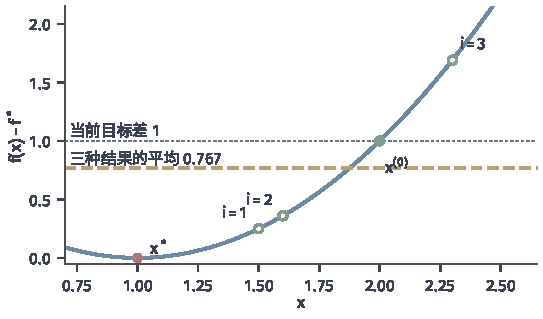
\includegraphics[width=92mm]{figures/05-optimization/05-stochastic-optimization/matplotlib/sgd-single-step/figure.pdf}
  \caption{单步的三种结果。蓝线是目标差$(x-1)^2$，实心绿点是当前点$x^{(0)}=2$，空心绿点是抽到第$i$项后的新点，步长$\alpha=0.1$。第三项使目标差上升到$1.69$，其余两项使它下降。虚线是三种结果的平均$0.767$，低于当前目标差$1$。}
  \label{fig:sgd-single-step}
\end{BookInlineFigure}

式~\eqref{eq:sgd-one-step}给出的数值是相同的。这里$L=2$，$\lvert f'(2)\rvert=2$，条件方差由式~\eqref{eq:sgd-example-variance}是$38/3$，所以下降量和噪声项分别是
\[
 0.1\cdot(1-0.1)\cdot4=0.36,\qquad 0.01\cdot\frac{38}{3}\approx0.127.
\]
于是
\[
 1-0.36+0.127=0.767.
\]
目标是二次函数，下降引理取等号，理论值与实际值完全相同。

\subsection{步长调度}
\label{sec:sgd-step-schedule}

单步分析留下一个问题：步长选大了噪声项大，选小了下降量小，$\alpha^{(t)}$该如何随$t$变化？

\paragraph{固定步长：收敛到一个邻域}
先看步长不变时发生什么。在强凸目标上，初始误差按几何速度消退，噪声则把误差托在一个不为零的水平。

\begin{theorem}[固定步长的误差邻域]
\label{thm:sgd-constant-step}
设$f$的梯度$L$-Lipschitz且$f$是$\mu$强凸的，读数条件无偏，且沿迭代点$\sigma_t^2\leq\sigma^2$。若固定步长$0<\alpha\leq1/L$，则对所有$T\geq0$，
\begin{equation}
 \mathbb{E}[f(\bm{x}^{(T)})]-f^\star\leq(1-\alpha\mu)^T\bigl(f(\bm{x}^{(0)})-f^\star\bigr)+\frac{\alpha L\sigma^2}{2\mu}.
 \label{eq:sgd-constant-step}
\end{equation}
\end{theorem}

\begin{proof}
记$e_t=\mathbb{E}[f(\bm{x}^{(t)})]-f^\star$。因为$\alpha L\leq1$，所以$1-L\alpha/2\geq1/2$，式~\eqref{eq:sgd-one-step}给出
\[
 \mathbb{E}[f(\bm{x}^{(t+1)})\mid\mathcal{F}^{(t)}]\leq f(\bm{x}^{(t)})-\frac{\alpha}{2}\lVert\nabla f(\bm{x}^{(t)})\rVert_2^2+\frac{L\alpha^2}{2}\sigma^2.
\]

强凸性给出对任意$\bm{x},\bm{y}$成立的下界
\[
 f(\bm{y})\geq f(\bm{x})+\langle\nabla f(\bm{x}),\bm{y}-\bm{x}\rangle+\frac{\mu}{2}\lVert\bm{y}-\bm{x}\rVert_2^2.
\]
右端对$\bm{y}$最小化，最小值在$\bm{y}=\bm{x}-\nabla f(\bm{x})/\mu$处取得，所以
\[
 f^\star\geq f(\bm{x})-\frac{1}{2\mu}\lVert\nabla f(\bm{x})\rVert_2^2.
\]
这就是
\[
 \lVert\nabla f(\bm{x})\rVert_2^2\geq2\mu\bigl(f(\bm{x})-f^\star\bigr).
\]

把这个下界代入第一个不等式，两边减去$f^\star$，再取全期望~\eqref{eq:sgd-tower}，得到递推
\[
 e_{t+1}\leq(1-\alpha\mu)e_t+\frac{L\alpha^2\sigma^2}{2}.
\]

由$\alpha\mu\leq\mu/L\leq1$，系数$1-\alpha\mu$非负，递推可以展开$T$次，得到
\[
 e_T\leq(1-\alpha\mu)^Te_0+\frac{L\alpha^2\sigma^2}{2}\sum_{k=0}^{T-1}(1-\alpha\mu)^k.
\]
几何级数不超过$1/(\alpha\mu)$，代入即得式~\eqref{eq:sgd-constant-step}。
\end{proof}

式~\eqref{eq:sgd-constant-step}的第一项随$T$消退，第二项不消退，称为\term{噪声底}（noise floor）。三个条件各有作用：光滑性使下降引理可用，强凸性把梯度大小换算成目标差，方差上界控制每步的损失。去掉强凸性，这个几何递推就不成立；去掉方差上界，噪声项无法用常数控制。

\paragraph{例中的精确递推}
三项目标可以把期望完全算出来。令$\delta_t=x^{(t)}-1$，由$x^{(t+1)}-1=\delta_t-\alpha\hat{g}^{(t)}$和式~\eqref{eq:sgd-example-variance}，条件期望分别是
\[
 \mathbb{E}[\delta_{t+1}\mid\mathcal{F}^{(t)}]=(1-2\alpha)\delta_t,
\]
\[
 \mathbb{E}[\delta_{t+1}^2\mid\mathcal{F}^{(t)}]=\Bigl(1-4\alpha+\frac{14}{3}\alpha^2\Bigr)\delta_t^2-\frac{20}{3}\alpha^2\delta_t+\frac{56}{3}\alpha^2.
\]

当$\alpha<6/7$时，$\delta_t^2$的系数小于$1$，且$\mathbb{E}[\delta_t]\to0$。令$\mathbb{E}[\delta_t^2]$的稳态值为$s$，在第二式中取全期望并令$\mathbb{E}[\delta_t]=0$，它满足
\[
 \Bigl(4\alpha-\frac{14}{3}\alpha^2\Bigr)s=\frac{56}{3}\alpha^2.
\]
解得
\begin{equation}
 \lim_{t\to\infty}\mathbb{E}[f(x^{(t)})-f^\star]=\frac{28\alpha}{6-7\alpha}.
 \label{eq:sgd-example-floor}
\end{equation}
$\alpha=0.1$时噪声底约为$0.528$，$\alpha=0.02$时约为$0.096$。

\begin{BookInlineFigure}
  \centering
  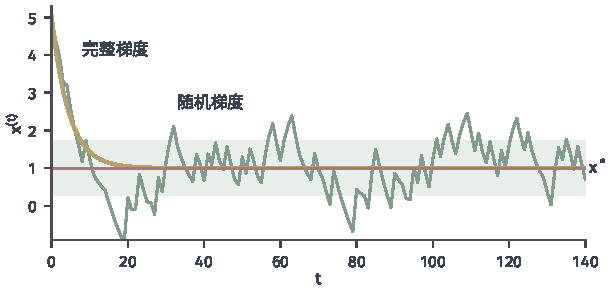
\includegraphics[width=104mm]{figures/05-optimization/05-stochastic-optimization/matplotlib/sgd-sample-path/figure.pdf}
  \caption{三项目标上从$x^{(0)}=5$出发，步长$\alpha=0.1$（种子固定）的一条路径。绿线是随机梯度，黄线是完整梯度，红线是$x^\star=1$。绿底带的半宽是式~\eqref{eq:sgd-example-floor}的平方根$0.727$，即稳态下均方根偏差。}
  \label{fig:sgd-sample-path}
\end{BookInlineFigure}

图~\ref{fig:sgd-sample-path}是一条实际路径。开始的十几步里绿线和黄线几乎重合：离解很远时信号强于噪声，抽到哪一项都往下走。之后黄线停在解上，绿线在一条带内不停抖动，这条带就是噪声底的样子。

\paragraph{固定、递减与分段}
固定步长的两部分误差互相拉扯：大的$\alpha$使初始误差消得快，噪声底却高；小的$\alpha$相反。要想噪声底趋于零，步长就得逐渐减小。

经典的递减条件是
\begin{equation}
 \sum_{t=0}^{\infty}\alpha^{(t)}=\infty,\qquad\sum_{t=0}^{\infty}(\alpha^{(t)})^2<\infty.
 \label{eq:sgd-robbins-monro}
\end{equation}
第一个要求表示累计可走的距离没有上限，初始点再远也到得了；第二个要求表示噪声积累的总量有限\scite{math-robbins1951stochastic}。例如$\alpha^{(t)}=c/(t+t_0)$同时满足两者。

分段调整介于两者之间：先用较大的步长，到达噪声底后减半，再走一段。每段把噪声底压低一半，代价是每段需要的步数翻倍。图~\ref{fig:sgd-step-schedules}(a)比较了几种调度，图中的曲线由递推精确算出。

\begin{BookInlineFigure}
  \centering
  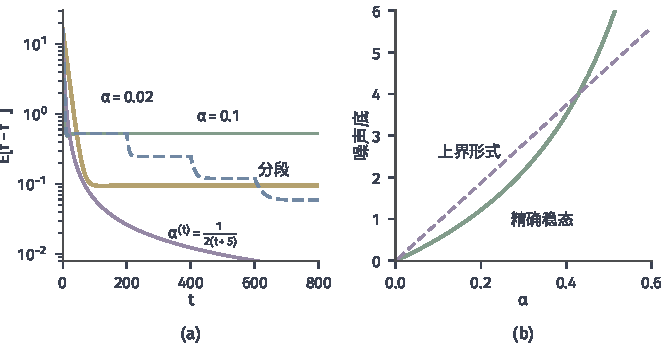
\includegraphics[width=112mm]{figures/05-optimization/05-stochastic-optimization/matplotlib/sgd-step-schedules/figure.pdf}
  \caption{三项目标的步长调度，由精确递推算出，$x^{(0)}=5$。(a)绿线和黄线是固定步长$0.1$和$0.02$，紫线是$\alpha^{(t)}=1/(2(t+5))$，蓝色虚线是从$0.1$起每$200$步减半。固定步长最后变平，大步长到得早而停得高；递减步长持续下降。(b)绿线是噪声底的精确值~\eqref{eq:sgd-example-floor}，紫色虚线是式~\eqref{eq:sgd-constant-step}第二项取$\sigma^2=56/3$的形式；后者只代入最优点处的方差，并非严格上界。步长较大时迭代离解较远，实际方差更大，绿线超过虚线。}
  \label{fig:sgd-step-schedules}
\end{BookInlineFigure}

\paragraph{时间单位}
调度写成$t$的函数时，要说明$t$计的是什么。常见的单位有三种：更新次数、读取的样本量、完整遍历的轮数。批量为$B$、项数为$N$时，一轮是$N/B$次更新，读取$N$个样本。

同一句“每200步减半”，用更新次数计时，批量改变后读取量不同；用样本量计时，批量改变后更新次数不同。批量、并行度或数据量一变，换算不当的调度含义就变了。式~\eqref{eq:sgd-constant-step}和式~\eqref{eq:sgd-robbins-monro}中的$t$都是更新次数。

\paragraph{步长依赖本轮读数时}
前面一直要求$\alpha^{(t)}$在抽样之前确定。步长若依赖本轮读数，$\mathbb{E}[\alpha^{(t)}\hat{\bm{g}}^{(t)}\mid\mathcal{F}^{(t)}]$不再等于$\alpha^{(t)}\nabla f(\bm{x}^{(t)})$，因为步长和方向相关。

在三项目标上看一个具体的后果。取只保留读数符号的规则，步长$\alpha/\lvert\hat{g}\rvert$，每步走固定距离。在$x=0.5$处，三个读数是$3.5,1,-7.5$，真梯度是$-1$，应该向右走。这三个读数的符号是两正一负，平均更新是
\[
 -\alpha\cdot\frac{1+1-1}{3}=-\frac{\alpha}{3},
\]
平均向左走，方向错了。

\begin{BookInlineFigure}
  \centering
  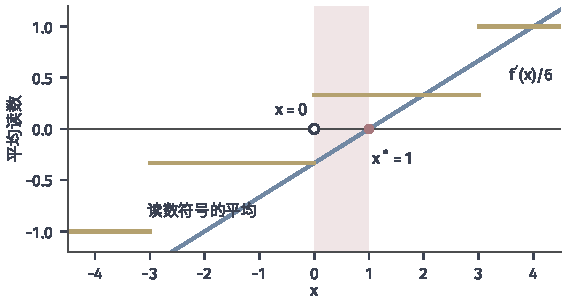
\includegraphics[width=96mm]{figures/05-optimization/05-stochastic-optimization/matplotlib/sgd-normalized-bias/figure.pdf}
  \caption{步长与读数相关时平均方向可能错误。蓝线是真梯度$f'(x)$按比例缩小$6$倍，零点是$x^\star=1$；黄色阶梯是三个读数符号的平均，零点是$x=0$。红底区间$(0,1)$内两者异号，按读数符号走的平均方向与真梯度相反。}
  \label{fig:sgd-normalized-bias}
\end{BookInlineFigure}

图~\ref{fig:sgd-normalized-bias}说明了问题的严重性：这条规则的平均动力学的零点是$x=0$，即各项最小点$-3,0,3$的中位数，而不是$x^\star=1$。缩小$\alpha$也改变不了这一点，因为偏差存在于平均方向之中。依赖读数的步长并非都不能用，后文讨论的方法多属于这一类，但必须分别分析步长与方向的相关性。

\subsection{凸目标的误差与输出}
\label{sec:sgd-convex}

前面的噪声底结论依赖强凸性。对一般的凸目标，$f-f^\star$与梯度大小没有固定的换算关系，下降引理的路线走不通。这一小节换一个量来追踪：到最优解的距离。

\paragraph{距离递推与平均点}
距离的好处是展开之后能用凸性。把更新代入$\lVert\bm{x}^{(t+1)}-\bm{x}^\star\rVert_2^2$，内积项由凸性转成目标差，所得到的结论是对迭代点的加权和成立的。

为了从加权和回到一个点，需要Jensen不等式：若$f$凸，$\lambda_t\geq0$，$\sum_t\lambda_t=1$，则
\[
 f\Bigl(\sum_t\lambda_t\bm{x}^{(t)}\Bigr)\leq\sum_t\lambda_tf(\bm{x}^{(t)}).
\]
两个点的情形就是凸函数的定义，多个点时对点数作归纳即得。

\begin{theorem}[凸目标的加权平均点]
\label{thm:sgd-convex}
设$f$凸且可微，存在最小点$\bm{x}^\star$，读数条件无偏，且沿迭代点读数的条件二阶矩不超过$G^2$，步长$\alpha^{(t)}>0$事先确定。记$R=\lVert\bm{x}^{(0)}-\bm{x}^\star\rVert_2$，$A_T=\sum_{t=0}^{T-1}\alpha^{(t)}$，加权平均点
\begin{equation}
 \bar{\bm{x}}^{(T)}=\frac{1}{A_T}\sum_{t=0}^{T-1}\alpha^{(t)}\bm{x}^{(t)}.
 \label{eq:sgd-weighted-average}
\end{equation}
则
\begin{equation}
 \mathbb{E}[f(\bar{\bm{x}}^{(T)})]-f^\star\leq\frac{R^2+G^2\sum_{t=0}^{T-1}(\alpha^{(t)})^2}{2A_T}.
 \label{eq:sgd-convex-bound}
\end{equation}
\end{theorem}

\begin{proof}
记$d_t$为$\lVert\bm{x}^{(t)}-\bm{x}^\star\rVert_2^2$的期望。展开平方，得到
\[
 \lVert\bm{x}^{(t+1)}-\bm{x}^\star\rVert_2^2=\lVert\bm{x}^{(t)}-\bm{x}^\star\rVert_2^2-2\alpha^{(t)}\langle\hat{\bm{g}}^{(t)},\bm{x}^{(t)}-\bm{x}^\star\rangle+(\alpha^{(t)})^2\lVert\hat{\bm{g}}^{(t)}\rVert_2^2.
\]

取$\mathbb{E}[\cdot\mid\mathcal{F}^{(t)}]$。$\bm{x}^{(t)}-\bm{x}^\star$由历史确定，内积项由条件无偏变成$\langle\nabla f(\bm{x}^{(t)}),\bm{x}^{(t)}-\bm{x}^\star\rangle$。凸性给出
\[
 \langle\nabla f(\bm{x}^{(t)}),\bm{x}^{(t)}-\bm{x}^\star\rangle\geq f(\bm{x}^{(t)})-f^\star.
\]

再用二阶矩的上界并取全期望，得到递推
\[
 d_{t+1}\leq d_t-2\alpha^{(t)}\bigl(\mathbb{E}[f(\bm{x}^{(t)})]-f^\star\bigr)+(\alpha^{(t)})^2G^2.
\]

对$t=0,\ldots,T-1$求和，左右的$d_t$逐项相消，再丢掉非负的$d_T$，得到
\[
 2\sum_{t=0}^{T-1}\alpha^{(t)}\bigl(\mathbb{E}[f(\bm{x}^{(t)})]-f^\star\bigr)\leq R^2+G^2\sum_{t=0}^{T-1}(\alpha^{(t)})^2.
\]

两边除以$2A_T$，并对$\lambda_t=\alpha^{(t)}/A_T$使用Jensen不等式，即得式~\eqref{eq:sgd-convex-bound}。
\end{proof}

固定步长$\alpha$时，式~\eqref{eq:sgd-convex-bound}的右端是$R^2/(2\alpha T)+\alpha G^2/2$。对$\alpha$求最小，取$\alpha=R/(G\sqrt{T})$，得到
\begin{equation}
 \mathbb{E}[f(\bar{\bm{x}}^{(T)})]-f^\star\leq\frac{RG}{\sqrt{T}}.
 \label{eq:sgd-convex-rate}
\end{equation}
要把目标差减小十倍，步数要增加一百倍。

二阶矩的上界$G^2$包含了梯度本身，在全空间常常不成立。若$f$还有$L$-Lipschitz梯度，条件可以放宽为条件方差不超过$\sigma^2$。在凸的$L$-光滑函数上，从$\bm{x}$走一步$\bm{x}-\nabla f(\bm{x})/L$，由下降引理，
\[
 f^\star\leq f(\bm{x})-\frac{1}{2L}\lVert\nabla f(\bm{x})\rVert_2^2.
\]
于是梯度大小被目标差控制，读数的二阶矩满足
\[
 \mathbb{E}[\lVert\hat{\bm{g}}^{(t)}\rVert_2^2\mid\mathcal{F}^{(t)}]\leq2L\bigl(f(\bm{x}^{(t)})-f^\star\bigr)+\sigma^2.
\]

把它代入上面的递推，当$\alpha\leq1/(2L)$时，由$1-\alpha L\geq1/2$，同样的求和给出
\begin{equation}
 \mathbb{E}[f(\bar{\bm{x}}^{(T)})]-f^\star\leq\frac{R^2}{\alpha T}+\alpha\sigma^2.
 \label{eq:sgd-convex-smooth}
\end{equation}
取$\alpha=\min\{1/(2L),R/(\sigma\sqrt{T})\}$，右端不超过$2LR^2/T+2R\sigma/\sqrt{T}$。第一项是完整梯度下降的速率，第二项是噪声带来的代价；$\sigma=0$时退回确定情形。

\paragraph{强凸性的改善}
强凸性使距离递推有了收缩，步长可以取到$1/t$的量级。

\begin{theorem}[强凸目标的递减步长]
\label{thm:sgd-strong-decay}
设$f$可微且$\mu$强凸，读数条件无偏，沿迭代点读数的条件二阶矩不超过$G^2$，$\alpha^{(t)}=1/(\mu(t+1))$。则对所有$T\geq1$，
\begin{equation}
 \mathbb{E}[\lVert\bm{x}^{(T)}-\bm{x}^\star\rVert_2^2]\leq\frac{G^2}{\mu^2T}.
 \label{eq:sgd-strong-rate}
\end{equation}
\end{theorem}

\begin{proof}
强凸下界中分别取$(\bm{x},\bm{x}^\star)$和$(\bm{x}^\star,\bm{x})$，相加并用$\nabla f(\bm{x}^\star)=\bm{0}$，得到
\[
 \langle\nabla f(\bm{x}),\bm{x}-\bm{x}^\star\rangle\geq\mu\lVert\bm{x}-\bm{x}^\star\rVert_2^2.
\]
沿用定理~\ref{thm:sgd-convex}证明中的展开，得到
\[
 d_{t+1}\leq(1-2\alpha^{(t)}\mu)d_t+(\alpha^{(t)})^2G^2=\Bigl(1-\frac{2}{t+1}\Bigr)d_t+\frac{G^2}{\mu^2(t+1)^2}.
\]

对$T$作归纳。$T=1$时，取$t=0$，系数是$-1$，由$d_0\geq0$有$d_1\leq G^2/\mu^2$，结论成立。

设$d_t\leq G^2/(\mu^2t)$，其中$t\geq1$，此时系数$1-2/(t+1)$非负。代入递推，得到
\[
 d_{t+1}\leq\frac{G^2}{\mu^2}\Bigl[\frac{t-1}{t(t+1)}+\frac{1}{(t+1)^2}\Bigr].
\]

只需证明方括号不超过$1/(t+1)$，即$\tfrac{t-1}{t}+\tfrac{1}{t+1}\leq1$。这等价于$\tfrac{1}{t+1}\leq\tfrac{1}{t}$，成立。
\end{proof}

强凸假设和全空间的$G^2$是矛盾的，因为强凸函数的梯度无界。定理中的条件要理解为迭代点在有界集内，通常由投影到有界闭凸集来保证，投影不增大到$\bm{x}^\star$的距离，上面的递推继续成立。

把结论总结成对比：

\begin{BookInlineTable}
  \centering
  \begin{tabular}{lll}
    \toprule
    条件 & 步长 & 期望误差\\
    \midrule
    凸，二阶矩有界 & $\dfrac{R}{G\sqrt{T}}$ & 平均点目标差$\dfrac{RG}{\sqrt{T}}$\\\addlinespace[2.5mm]
    凸，光滑，方差有界 & $\min\Bigl\{\dfrac{1}{2L},\dfrac{R}{\sigma\sqrt{T}}\Bigr\}$ & 平均点目标差$\dfrac{2LR^2}{T}+\dfrac{2R\sigma}{\sqrt{T}}$\\\addlinespace[2.5mm]
    强凸，二阶矩有界 & $\dfrac{1}{\mu(t+1)}$ & 末点距离平方$\dfrac{G^2}{\mu^2T}$\\\addlinespace[2.5mm]
    强凸，光滑，方差有界 & 固定，$\alpha\leq\dfrac1L$ & 末点目标差，含噪声底\\
    \bottomrule
  \end{tabular}
  \caption{本小节及上一小节的保证。表中“末点”指最后一个迭代点，“光滑”指梯度$L$-Lipschitz。前两行的结论针对平均点，后两行针对末点。}
  \label{tab:sgd-rates}
\end{BookInlineTable}

\paragraph{最后一点与平均点}
定理~\ref{thm:sgd-convex}的保证属于平均点，不能搬到任意一个迭代点上。平均值小只说明大多数项小：序列$0,0,\ldots,0,3$的平均可以任意小，而最后一项是$3$。一般凸目标上最后一点的保证需要单独证明，所得的速率通常比平均点差，具体分析较长，读者可查阅专门的文献。

\begin{BookInlineFigure}
  \centering
  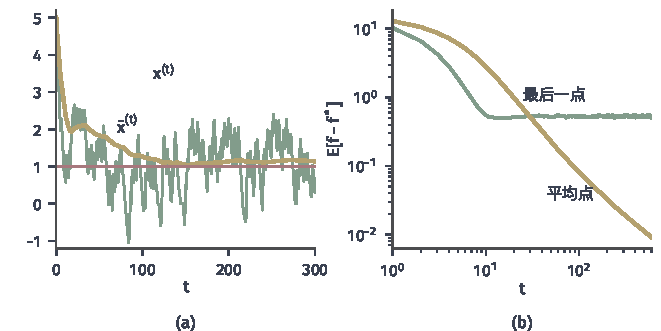
\includegraphics[width=112mm]{figures/05-optimization/05-stochastic-optimization/matplotlib/sgd-average-vs-last/figure.pdf}
  \caption{三项目标上固定步长$\alpha=0.1$，从$x^{(0)}=5$出发。(a)同一条路径上最后一点$x^{(t)}$（绿）和从头算起的平均点$\bar{x}^{(t)}$（黄），红线是$x^\star$。(b)$4000$次独立运行的平均目标差（种子固定），两轴取对数。$t=600$时最后一点的目标差约为$0.53$，平均点约为$0.009$。}
  \label{fig:sgd-average-vs-last}
\end{BookInlineFigure}

在三项目标上平均的作用很明显。图~\ref{fig:sgd-average-vs-last}(a)的绿线一直在抖，黄线很快贴近解。(b)说明最后一点停在噪声底$0.53$，平均点的目标差继续下降。原因是抖动在解的两侧来回，平均时相互抵消，而初始段的影响被越来越多的项稀释。平均点要付出的代价是多存一个向量，并且受早期迭代点的拖累，因此实践中也常只平均后面一段。

\subsection{非凸目标的误差与输出}
\label{sec:sgd-nonconvex}

目标非凸时，到最小点的距离既不能保证下降，也可能不止一个最小点。只能回到单步下降，评价的量也要换成梯度大小。

\paragraph{累加下降量}
式~\eqref{eq:sgd-one-step}不需要凸性，把它沿$t$累加，左边望远镜相消，剩下函数值的总下降量，它受目标下界限制。

\begin{theorem}[非凸目标的平均平方梯度]
\label{thm:sgd-nonconvex}
设$f$有下界$f_{\inf}$，梯度$L$-Lipschitz，读数条件无偏且沿迭代点$\sigma_t^2\leq\sigma^2$，步长事先确定且$0<\alpha^{(t)}\leq1/L$。记$\Delta=f(\bm{x}^{(0)})-f_{\inf}$，$A_T=\sum_{t=0}^{T-1}\alpha^{(t)}$。则
\begin{equation}
 \frac{1}{A_T}\sum_{t=0}^{T-1}\alpha^{(t)}\mathbb{E}[\lVert\nabla f(\bm{x}^{(t)})\rVert_2^2]\leq\frac{2\Delta+L\sigma^2\sum_{t=0}^{T-1}(\alpha^{(t)})^2}{A_T}.
 \label{eq:sgd-nonconvex-bound}
\end{equation}
\end{theorem}

\begin{proof}
由$\alpha^{(t)}L\leq1$，式~\eqref{eq:sgd-one-step}的系数$1-L\alpha^{(t)}/2\geq1/2$。取全期望，得到
\[
 \frac{\alpha^{(t)}}{2}\mathbb{E}[\lVert\nabla f(\bm{x}^{(t)})\rVert_2^2]\leq\mathbb{E}[f(\bm{x}^{(t)})]-\mathbb{E}[f(\bm{x}^{(t+1)})]+\frac{L(\alpha^{(t)})^2}{2}\sigma^2.
\]

对$t=0,\ldots,T-1$求和，函数值逐项相消，只剩$f(\bm{x}^{(0)})-\mathbb{E}[f(\bm{x}^{(T)})]$，由下界，它不超过$\Delta$。于是
\[
 \frac12\sum_{t=0}^{T-1}\alpha^{(t)}\mathbb{E}[\lVert\nabla f(\bm{x}^{(t)})\rVert_2^2]\leq\Delta+\frac{L\sigma^2}{2}\sum_{t=0}^{T-1}(\alpha^{(t)})^2.
\]
两边乘以$2/A_T$，即得式~\eqref{eq:sgd-nonconvex-bound}。
\end{proof}

固定步长时，右端是$2\Delta/(\alpha T)+L\sigma^2\alpha$。取
\[
 \alpha=\min\Bigl\{\frac1L,\ \sqrt{\frac{2\Delta}{L\sigma^2T}}\Bigr\},
\]
并利用$1/\alpha$不超过两个倒数之和，得到
\begin{equation}
 \frac{1}{T}\sum_{t=0}^{T-1}\mathbb{E}[\lVert\nabla f(\bm{x}^{(t)})\rVert_2^2]\leq\frac{2L\Delta}{T}+2\sqrt{\frac{2L\Delta\sigma^2}{T}}.
 \label{eq:sgd-nonconvex-rate}
\end{equation}

\paragraph{按权重随机返回}
式~\eqref{eq:sgd-nonconvex-bound}的左端是平均，还不是某个点的性质。非凸时平均点没有Jensen不等式可用，点的平均甚至可能落在山顶上。解决办法是把平均变成一个随机的点：以概率$\alpha^{(t)}/A_T$抽取下标$\tau$，返回$\bm{x}^{(\tau)}$。由全期望公式，
\[
 \mathbb{E}[\lVert\nabla f(\bm{x}^{(\tau)})\rVert_2^2]=\frac{1}{A_T}\sum_{t=0}^{T-1}\alpha^{(t)}\mathbb{E}[\lVert\nabla f(\bm{x}^{(t)})\rVert_2^2].
\]
所以左端是这个随机输出的期望平方梯度。

用一个能实际计算的非凸例子来看。取$f_i(x)=1-\cos x+c_ix$，$(c_1,c_2,c_3)=(-2,0,2)$，则
\[
 f(x)=1-\cos x,\qquad f_i'(x)=\sin x+c_i.
\]
这里$f_{\inf}=0$，$L=1$，条件方差恰好是常数$\sigma^2=8/3$，所有假设都严格成立。取$x^{(0)}=2.5$，$\alpha=0.1$，$T=800$，则$\Delta=1-\cos2.5\approx1.80$，上界是
\[
 \frac{2\cdot1.80}{0.1\cdot800}+1\cdot\frac83\cdot0.1\approx0.045+0.267=0.312.
\]

\begin{BookInlineFigure}
  \centering
  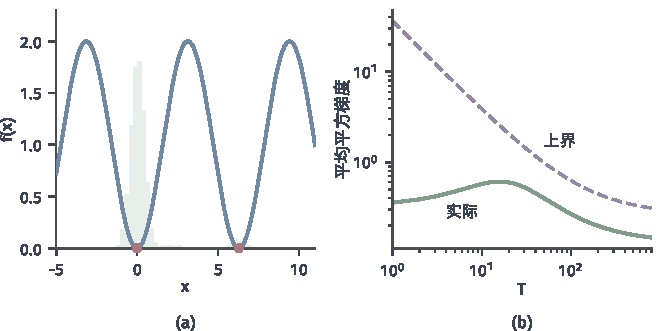
\includegraphics[width=112mm]{figures/05-optimization/05-stochastic-optimization/matplotlib/sgd-nonconvex-output/figure.pdf}
  \caption{非凸目标$f(x)=1-\cos x$上$6000$次独立运行的随机梯度方法（种子固定），$x^{(0)}=2.5$，$\alpha=0.1$。(a)蓝线是目标函数，红点是最小点$x=0$和$2\pi$，绿底直方图是$T=800$时按权重随机返回的点的分布（纵向已缩放）。(b)绿线是$T$步内平方梯度的平均，紫色虚线是式~\eqref{eq:sgd-nonconvex-bound}的上界，两轴取对数。}
  \label{fig:sgd-nonconvex-output}
\end{BookInlineFigure}

图~\ref{fig:sgd-nonconvex-output}(b)显示实际平均约为$0.147$，低于上界$0.312$。上界的第二项$\alpha L\sigma^2$对应的正是噪声底，这个上界在$T$增大时不趋于零，要趋于零必须同时缩小$\alpha$。图(a)中大多数返回点集中在$x=0$附近，少数越过山峰到了$2\pi$附近。

\paragraph{这个结论不说明什么}
式~\eqref{eq:sgd-nonconvex-bound}只评价一阶驻定。小梯度的点可能在鞍点或平坦的高处，它与局部极小的距离没有被保证；能否离开鞍点是第~\ref{chap:saddle-points}章的主题。

它也是期望界，不是逐路径保证。由Markov不等式，对$\varepsilon>0$，
\[
 \mathbb{P}\bigl(\lVert\nabla f(\bm{x}^{(\tau)})\rVert_2^2\geq\varepsilon\bigr)\leq\frac{\mathbb{E}[\lVert\nabla f(\bm{x}^{(\tau)})\rVert_2^2]}{\varepsilon},
\]
只给出一次运行的概率控制。随着$t\to\infty$路径本身的行为，例如几乎处处收敛，需要鞅收敛等工具，可参考\BookChapterRef{chap:discrete-time-stochastic-processes}{卷九第3章“离散时间随机过程”}。

\subsection{随机邻近梯度}
\label{sec:sgd-proximal}

目标带非光滑项时，上面的更新不能直接用。本小节要解决的问题是：非光滑项确定而光滑项需要抽样，邻近步该怎样接上随机读数？

\paragraph{主要思想}
设复合目标$F(\bm{x})=f(\bm{x})+h(\bm{x})$，其中$f$是光滑的有限和或期望目标，$h$是适当、下半连续的凸函数，且邻近映射可以计算。\term{随机邻近梯度法}（stochastic proximal gradient method）只对光滑部分抽样，$h$则每步精确处理：
\begin{equation}
 \bm{x}^{(t+1)}=\operatorname{prox}_{\alpha^{(t)}h}\bigl(\bm{x}^{(t)}-\alpha^{(t)}\hat{\bm{g}}^{(t)}\bigr),
 \label{eq:sgd-prox-update}
\end{equation}
其中邻近映射的定义和计算见第~\ref{chap:nonsmooth-composite-optimization}章。$h$不参与抽样，只在邻近步中出现，这样$\hat{\bm{g}}^{(t)}$的条件无偏性只关系到$f$。

\paragraph{计算过程}
在三项目标上加$h(x)=\gamma\lvert x\rvert$，取$\gamma=1$。复合目标的最优解满足$2x-2+\gamma=0$，所以$x^\star=0.5$，它是正的，与$\lvert x\rvert$的导数取$+1$相符。邻近映射是软阈值：
\[
 \operatorname{prox}_{\alpha h}(z)=\operatorname{sign}(z)\max\{\lvert z\rvert-\alpha\gamma,0\}.
\]
变量与第~\ref{sec:sgd-basic}小节相同，多一个非光滑项的参数。每轮更新三步：抽样下标$i^{(t)}$，走一步随机梯度得到中间点$\bm{z}^{(t)}$，求$\bm{z}^{(t)}$的邻近点作为$\bm{x}^{(t+1)}$。

例中取$x^{(t)}=0.2$，$\alpha=0.1$，阈值是$0.1$。三项读数分别是$3.2,0.4,-8.4$，完整梯度是$-1.6$。走完梯度步的三种结果是
\[
 z=-0.12,\quad z=0.16,\quad z=1.04,
\]
对应的邻近点分别是
\[
 -0.02,\quad 0.06,\quad 0.94.
\]

\paragraph{随机更新的均值不等于精确更新}
三个邻近点的平均是$0.327$。精确更新则先平均梯度，$z=0.36$，邻近点是$0.26$。两者不相等。

\begin{BookInlineFigure}
  \centering
  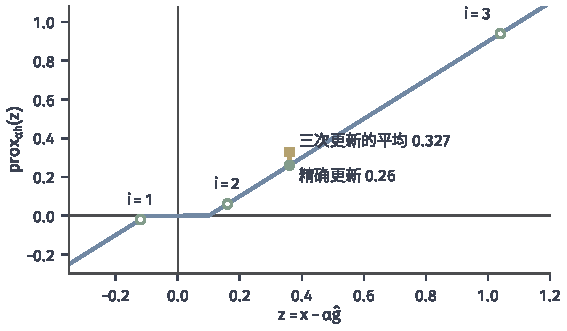
\includegraphics[width=96mm]{figures/05-optimization/05-stochastic-optimization/matplotlib/sgd-prox-bias/figure.pdf}
  \caption{邻近映射的非线性。蓝线是阈值为$0.1$的软阈值函数。三个空心点是三种读数对应的结果。实心绿点是先平均$z$再求邻近点的精确更新，黄方块是三次邻近点的平均。两点之差来自软阈值在零附近的弯折。}
  \label{fig:sgd-prox-bias}
\end{BookInlineFigure}

图~\ref{fig:sgd-prox-bias}说明了原因：邻近映射是非线性的，先平均再映射与先映射再平均结果不同。所以即使$\hat{\bm{g}}^{(t)}$条件无偏，随机更新的均值一般也不等于精确更新。这就是不能直接沿用无偏分析的地方。

\paragraph{误差的评价}
凸情形用复合目标差评价。证明的关键是引入精确更新点，把含噪声的内积拆开。

\begin{theorem}[随机邻近梯度的平均点]
\label{thm:sgd-prox}
设$f$凸且梯度$L$-Lipschitz，$h$适当、下半连续、凸，$F=f+h$有最小点$\bm{x}^\star$。读数条件无偏，沿迭代点$\sigma_t^2\leq\sigma^2$，固定步长$0<\alpha\leq1/L$。记$R=\lVert\bm{x}^{(0)}-\bm{x}^\star\rVert_2$，$\bar{\bm{x}}^{(T)}$为$\bm{x}^{(1)},\ldots,\bm{x}^{(T)}$的算术平均，则
\begin{equation}
 \mathbb{E}[F(\bar{\bm{x}}^{(T)})]-F(\bm{x}^\star)\leq\frac{R^2}{2\alpha T}+\alpha\sigma^2.
 \label{eq:sgd-prox-bound}
\end{equation}
\end{theorem}

\begin{proof}
证明中把当前点和下一点记为$\bm{x},\bm{x}^+$，噪声记为$\bm{\zeta}$，比较点$\bm{u}$取为$\bm{x}^\star$。由下降引理和$f$的凸性，
\[
 f(\bm{x}^+)\leq f(\bm{u})+\langle\nabla f(\bm{x}),\bm{x}^+-\bm{u}\rangle+\frac{L}{2}\lVert\bm{x}^+-\bm{x}\rVert_2^2.
\]

邻近点的最优性条件说明$(\bm{x}-\alpha\hat{\bm{g}}^{(t)}-\bm{x}^+)/\alpha$是$h$在$\bm{x}^+$处的次梯度，于是
\[
 h(\bm{x}^+)\leq h(\bm{u})-\langle\hat{\bm{g}}^{(t)},\bm{x}^+-\bm{u}\rangle+\frac{1}{\alpha}\langle\bm{x}-\bm{x}^+,\bm{x}^+-\bm{u}\rangle.
\]

把两式相加。对最后的内积使用恒等式
\[
 2\langle\bm{x}-\bm{x}^+,\bm{x}^+-\bm{u}\rangle=\lVert\bm{x}-\bm{u}\rVert_2^2-\lVert\bm{x}^+-\bm{u}\rVert_2^2-\lVert\bm{x}^+-\bm{x}\rVert_2^2.
\]
由$\alpha\leq1/L$，$\lVert\bm{x}^+-\bm{x}\rVert_2^2$的系数$L/2-1/(2\alpha)$非正，可以丢掉，得到
\[
 F(\bm{x}^+)-F(\bm{u})\leq\frac{\lVert\bm{x}-\bm{u}\rVert_2^2-\lVert\bm{x}^+-\bm{u}\rVert_2^2}{2\alpha}-\langle\bm{\zeta},\bm{x}^+-\bm{u}\rangle.
\]

最后一项里$\bm{x}^+$依赖$\bm{\zeta}$，条件期望不为零。这里引入用真梯度算出的精确更新点
\[
 \bm{p}=\operatorname{prox}_{\alpha h}\bigl(\bm{x}-\alpha\nabla f(\bm{x})\bigr).
\]
它由历史确定，于是
\[
 \mathbb{E}[\langle\bm{\zeta},\bm{p}-\bm{u}\rangle\mid\mathcal{F}^{(t)}]=0.
\]

邻近映射是非扩张的，两个输入相差$\alpha\bm{\zeta}$，所以$\bm{x}^+$与$\bm{p}$的距离不超过$\alpha\lVert\bm{\zeta}\rVert_2$。再由Cauchy--Schwarz不等式，
\[
 -\langle\bm{\zeta},\bm{x}^+-\bm{p}\rangle\leq\alpha\lVert\bm{\zeta}\rVert_2^2.
\]

取条件期望，得到
\[
 \mathbb{E}[F(\bm{x}^+)\mid\mathcal{F}^{(t)}]-F(\bm{u})\leq\frac{\lVert\bm{x}-\bm{u}\rVert_2^2-\mathbb{E}[\lVert\bm{x}^+-\bm{u}\rVert_2^2\mid\mathcal{F}^{(t)}]}{2\alpha}+\alpha\sigma^2.
\]
取全期望后对$t=0,\ldots,T-1$求和，距离项逐项相消，再除以$T$，并由$F$的凸性用Jensen不等式，即得式~\eqref{eq:sgd-prox-bound}。
\end{proof}

非凸的光滑部分要用另一种度量。精确邻近梯度映射是
\begin{equation}
 \bm{G}_\alpha(\bm{x})=\frac{1}{\alpha}\Bigl[\bm{x}-\operatorname{prox}_{\alpha h}\bigl(\bm{x}-\alpha\nabla f(\bm{x})\bigr)\Bigr],
 \label{eq:sgd-prox-mapping}
\end{equation}
$\bm{G}_\alpha(\bm{x})=\bm{0}$恰好是复合目标的驻点条件。把$\nabla f$换成读数就得到含噪声的读数，它不能代替驻点残差。例中$x=0.2$处$G_\alpha=(0.2-0.26)/0.1=-0.6$，而三次含噪读数是$2.2$，$1.4$，$-7.4$，平均$-1.27$，既不等于$-0.6$，也没有哪一次接近它。这种读数变小，不能说明当前点接近驻点。

\subsection{随机块更新}
\label{sec:sgd-block}

第~\ref{chap:block-optimization}章的分块方法每步只更新变量的一块。本节的方法每步只读一部分目标项。两者可以同时使用，这时要说清每种随机选择各带来什么。

\paragraph{两种随机选择}
把变量分成$J$块，第$j$块的偏梯度记为$\nabla_jf$，$\bm{U}_j$把第$j$块的向量放回全长向量的相应位置，其余分量补零。随机块更新在第$t$步选一块$j^{(t)}$，抽一项$i^{(t)}$，然后
\begin{equation}
 \bm{x}^{(t+1)}=\bm{x}^{(t)}-\alpha_{j^{(t)}}\bm{U}_{j^{(t)}}\nabla_{j^{(t)}}f_{i^{(t)}}(\bm{x}^{(t)}).
 \label{eq:sgd-block-update}
\end{equation}
选块是对变量抽样，选项是对目标项抽样，图~\ref{fig:sgd-block-item-grid}用一张二维表表示。

\begin{BookInlineFigure}
  \centering
  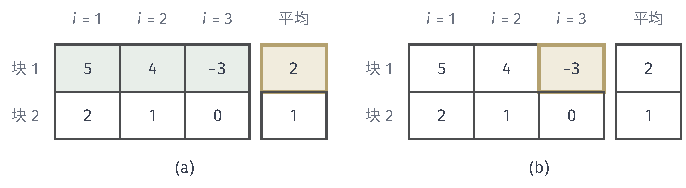
\includegraphics[width=112mm]{figures/05-optimization/05-stochastic-optimization/tikz/sgd-block-item-grid/figure.pdf}
  \caption{读取一次的范围。行是变量块，列是目标项，表中数字是第$i$项对第$j$块的偏导。(a)只随机选块：读完一行所有项（绿底），得到精确的偏梯度（黄框）。(b)同时选块和选项：只读一格（黄框），这个数是偏导的一次读数。}
  \label{fig:sgd-block-item-grid}
\end{BookInlineFigure}

用二元的例子把数字写出来。把贯穿例的$x$记作$x_1$，再加一个变量$x_2$，令第$i$项是
\[
 f_i(x_1,x_2)=\frac{a_i}{2}(x_1-b_i)^2+\frac12(x_2-c_i)^2,\qquad(c_1,c_2,c_3)=(-1,0,1).
\]
在$(2,1)$处，第一块的三个偏导是$5,4,-3$，平均$2$；第二块的三个偏导是$2,1,0$，平均$1$。

\paragraph{固定历史后的核对}
分两层取条件期望。先固定历史和选中的块$j$，只对目标项求平均，由式~\eqref{eq:sgd-uniform-mean}得到
\[
 \mathbb{E}\bigl[\nabla_jf_{i^{(t)}}(\bm{x}^{(t)})\mid\mathcal{F}^{(t)},j\bigr]=\nabla_jf(\bm{x}^{(t)}).
\]
所以给定块之后读数对这一块的偏梯度无偏，条件方差记为$\sigma_j^2$。这一条要求选项的抽样分布不依赖于这一步的读数。若先把各块的读数算出来，再选读数最大的块，结果就有偏。

对选中的块使用块光滑常数$L_j$，第~\ref{chap:block-optimization}章的块下降引理给出的单步界与式~\eqref{eq:sgd-one-step}同样推导：
\begin{equation}
 \begin{aligned}
 \mathbb{E}[f(\bm{x}^{(t+1)})\mid\mathcal{F}^{(t)},j]
 \leq{}&f(\bm{x}^{(t)})-\alpha_j\Bigl(1-\frac{L_j\alpha_j}{2}\Bigr)\lVert\nabla_jf(\bm{x}^{(t)})\rVert_2^2\\
 &+\frac{L_j\alpha_j^2}{2}\sigma_j^2.
 \end{aligned}
 \label{eq:sgd-block-one-step}
\end{equation}

\paragraph{两类随机性并存时}
再对块的选择求平均。取块均匀，$\alpha_j=1/L_j$，由式~\eqref{eq:sgd-block-one-step}，
\[
 \mathbb{E}[f(\bm{x}^{(t+1)})\mid\mathcal{F}^{(t)}]\leq f(\bm{x}^{(t)})-\frac{1}{J}\sum_{j=1}^{J}\frac{\lVert\nabla_jf(\bm{x}^{(t)})\rVert_2^2}{2L_j}+\frac{1}{J}\sum_{j=1}^{J}\frac{\sigma_j^2}{2L_j}.
\]
只随机选块时$\sigma_j=0$，退回第~\ref{chap:block-optimization}章的结论，读取一行的成本是$N$项对这一块的偏导。同时抽样时，一次更新只读一格，代价小得多，但多出噪声项，邻域和步长都要像上面那样处理。

步长也要按两种随机性分别考虑：块步长$\alpha_j$由块光滑常数决定，抽样噪声则要求更小的步长或方差控制。一个容易犯的错误是把噪声项算成所有块的方差之和，而每次其实只读一块；另一个错误是只对选项取期望，忘记选块也是随机的。例中在$(2,1)$处，选块均匀、$\alpha_j=0.1$时，平均更新量是
\[
 -\frac12\cdot0.1\cdot(2,1)=(-0.1,-0.05).
\]
这是两层平均的结果：选中第一块时第一个分量的平均更新是$-0.2$，第二个分量不变，第二块反过来。一次实际抽样中，比如选第一块、第三项，更新量是$(+0.3,0)$，这与平均方向相反，与第~\ref{sec:sgd-unbiased}小节的单项读数相反的情形相同。
